\documentclass{article}


% if you need to pass options to natbib, use, e.g.:
%     \PassOptionsToPackage{numbers, compress}{natbib}
% before loading neurips_2024


% ready for submission
\usepackage[final]{neurips_2024}


% to compile a preprint version, e.g., for submission to arXiv, add add the
% [preprint] option:
%     \usepackage[preprint]{neurips_2024}


% to compile a camera-ready version, add the [final] option, e.g.:
%     \usepackage[final]{neurips_2024}


% to avoid loading the natbib package, add option nonatbib:
%    \usepackage[nonatbib]{neurips_2024}


\usepackage[utf8]{inputenc} % allow utf-8 input
\usepackage[T1]{fontenc}    % use 8-bit T1 fonts
\usepackage{hyperref}       % hyperlinks
\usepackage{url}            % simple URL typesetting
\usepackage{booktabs}       % professional-quality tables
\usepackage{amsfonts}       % blackboard math symbols
\usepackage{nicefrac}       % compact symbols for 1/2, etc.
\usepackage{microtype}      % microtypography
\usepackage{xcolor}         % colors
\usepackage{graphicx}
\usepackage{pdflscape}


\title{Overcooked}


% The \author macro works with any number of authors. There are two commands
% used to separate the names and addresses of multiple authors: \And and \AND.
%
% Using \And between authors leaves it to LaTeX to determine where to break the
% lines. Using \AND forces a line break at that point. So, if LaTeX puts 3 of 4
% authors names on the first line, and the last on the second line, try using
% \AND instead of \And before the third author name.


\author{%
    Alessio Arcara\\
    University of Bologna\\
    \texttt{alessio.arcara@studio.unibo.it}
}


\begin{document}


\maketitle


\begin{abstract}
  The abstract paragraph should be indented \nicefrac{1}{2}~inch (3~picas) on
  both the left- and right-hand margins. Use 10~point type, with a vertical
  spacing (leading) of 11~points.  The word \textbf{Abstract} must be centered,
  bold, and in point size 12. Two line spaces precede the abstract. The abstract
  must be limited to one paragraph.
\end{abstract}

\section{Introduction}

Overcooked-AI\cite{carroll2020utilitylearninghumanshumanai} environment was designed a where the goal is to place three
onions in a pot, take the resulting soup on a plate and delivering it


that allows benchmark and evaluate
reinforcement learning (RL) agents on their ability to cooperate with unknown
partners in unfamiliarity environments
% overcooked e minifigura

This work chooses \textbf{Indipendent Proximal Policy Optimization (IPPO)} as
the learning algorithm for the cooperative multi-agent reinforcement learning
(MARL) problem. Under indipendent learning, a MARL problem is decomposed into
$n$ interdependent learning problems, which are solved independently by each
agent. Each agent treats the other agents as part of the environment and
learns its own policy and value function based solely on local observations.

While this approach is simple and scalable, it violates the stationarity
assumption required by Markov Decision Processes (MDPs), since the environment
dynamics change as other agents update their policies. As a result,
independent learning may suffer from non-stationarity.

Centralized training methods attempt to address non-stationarity by using
global information during training, either through joint policy learning or
centralized value functions. However, recent empirical results show that IPPO
can match or even outperform CTDE methods, such as QMIX and MAPPO
\cite{dewitt2020independentlearningneedstarcraft,
yu2022surprisingeffectivenessppocooperative}.

The clipped surrogate objective of PPO effectively mitigates non-stationarity
issues, making IPPO a simple and effective baseline for cooperative MARL,
without requiring a centralized critic conditioned on the global state or on
the concatenation of agents observations, as in MAPPO.

\section{Background}

\section{Methodology}

\subsection{Implementation}

\subsection{State Representation}

\subsection{Reward Shaping}

\subsection{Experiments}


\begin{figure}[ht]
    \centering
    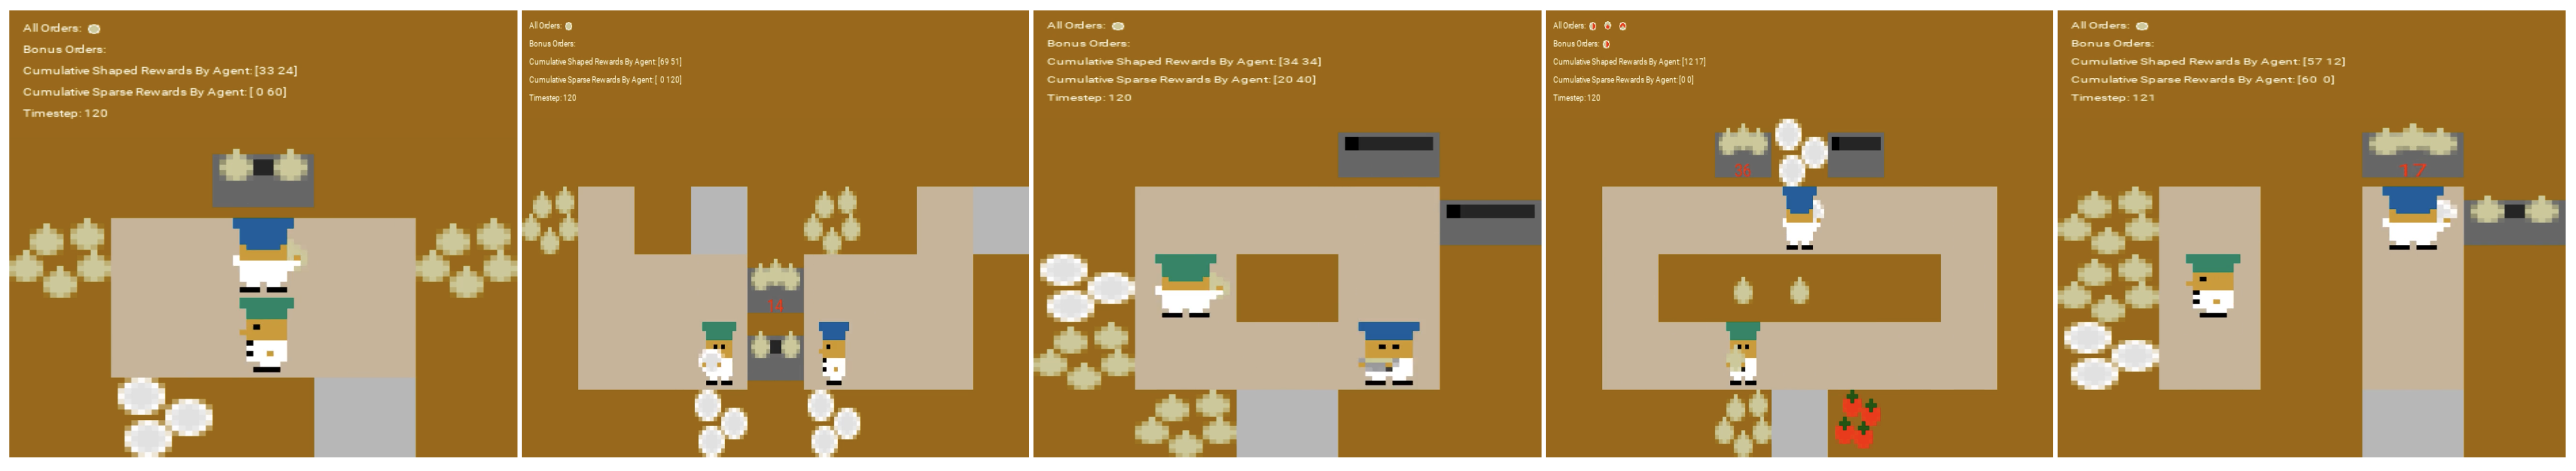
\includegraphics[width=\linewidth]{images/training_layouts}
    \caption{Training layouts: Cramped Room, Asymmetric Advantage,
    Coordination Ring, Counter Circuit, and Forced Coordination.}
    \label{fig:training_layouts}
\end{figure}

\subsubsection{Hardware \& Software} Experiments were conducted on a desktop
machine equipped with a 16-core CPU, 32 GB of RAM, and an NVIDIA GeForce RTX
3090 GPU used for both rollout collection and training updates. We developed
the implementation using \textbf{Jax} and \textbf{Flax}, which helped
significantly with computation speed. It is important to note that a Jax
implementation of the environment, such as the one available in JaxMARL, would
allow for much faster rollout collection. This phase was the main bottleneck
in our pipeline, as the GPU often remained underutilized while waiting for the
CPU to finish collecting rollouts. Although we avoided switching to a
Jax-native environment to align with the specific requirements of the project,
such a transition would be incredibly beneficial to maximize computational
throughput.

Furthermore, since the primary bottleneck is rollout collection, a
\textbf{vectorized environment} was utilized to run multiple environments in
parallel across separate processes using Gymnasium \texttt{AsyncVectorizeEnv}.
In this setting, the agent pair interacts simultaneously across $N$
environments, significantly increasing training throughput. The number of
environments was set to approximately the number of available CPU cores. It is
worth noting that a native Jax implementation would allow $N$ to be increased
by orders of magnitude.

By leveraging this setup, we achieved a training time of approximately 30
minutes per 10M steps. This allowed for extensive hyperparameter tuning with
Optuna within a highly reasonable timeframe.

\subsubsection{Hyperparameters Optimization}

We conducted hyperparameter optimization using \textbf{Optuna} over 50 trials,
with a total runtime of approximately 16 hours. The hyperparameter search used
the Tree-structured Parzen Estimator (TPE) to guide sampling toward promising
regions of the search space by modeling the performance of good and bad
configurations, while Hyperband was employed to efficiently allocate resources
and prune underperforming trials through early stopping. Full details are
reported in Appendix \ref{appendix:hpo}.

As shown in Figure \ref{fig:opt_history}, MLP models with featurized
environment encoding consistently outperformed CNNs with lossless environment
encoding, converging faster and achieving higher final returns.

The parallel coordinates plots (Figure~\ref{fig:parallel_coords}) show that
stable and high-performing configurations concentrate in a narrow region of
the hyperparameter space: an entropy coefficient of $0.01$–$0.05$, GAE
$\lambda$ between $0.9$ and $0.95$, 800-step rollout segments, and learning
rates of $10^{-4}$–$10^{-3}$. The MLP uses a 256-unit hidden layer. Sharing
parameters between agents consistently improved performance, whereas sharing a
backbone between the policy and value networks did not.

\subsubsection{Results}

\begin{table}[ht]
    \small
    \centering
    \setlength{\tabcolsep}{4pt} 
    \caption{Agent Pair Total Reward across different layouts (Average over 10
    episodes)}
    \begin{tabular}{l ccccc cc}
        \toprule
        & \multicolumn{5}{c}{\textbf{Training Layouts}} & \multicolumn{2}{c}{\textbf{Holdout Layouts}} \\
        \cmidrule(lr){2-6} \cmidrule(lr){7-8}
        
               & \textbf{Cramped} & \textbf{Asymm.} & \textbf{Coord.} & \textbf{Forced} & \textbf{Counter} & \textbf{Cramped} & \textbf{5x5} \\
                        & \textbf{Room}    & \textbf{Adv.}   & \textbf{Ring}   & \textbf{Coord.} & \textbf{Circuit} & \textbf{Tomato}  & \\
        \midrule

        Trained on all training layouts   & 220 & \underline{\textbf{460}} & \underline{\textbf{260}} & 260 & - & \underline{\textbf{315}} & - \\
        \midrule
        Trained on Cramped Room  & \underline{\textbf{240}} & - & - & - & - & - & - \\
        Trained on Asymm. Adv.   & - & \underline{\textbf{460}} & - & - & - & - & - \\
        Trained on Coord. Ring   & - & - & 200 & - & - & - & - \\
        Trained on Forced Coord. & - & - & - & \underline{\textbf{300}} & - & - & - \\
        Trained on Counter Circ. & - & - & - & - & - & - & - \\

        \bottomrule
    \end{tabular}
\end{table}

\begin{center}
    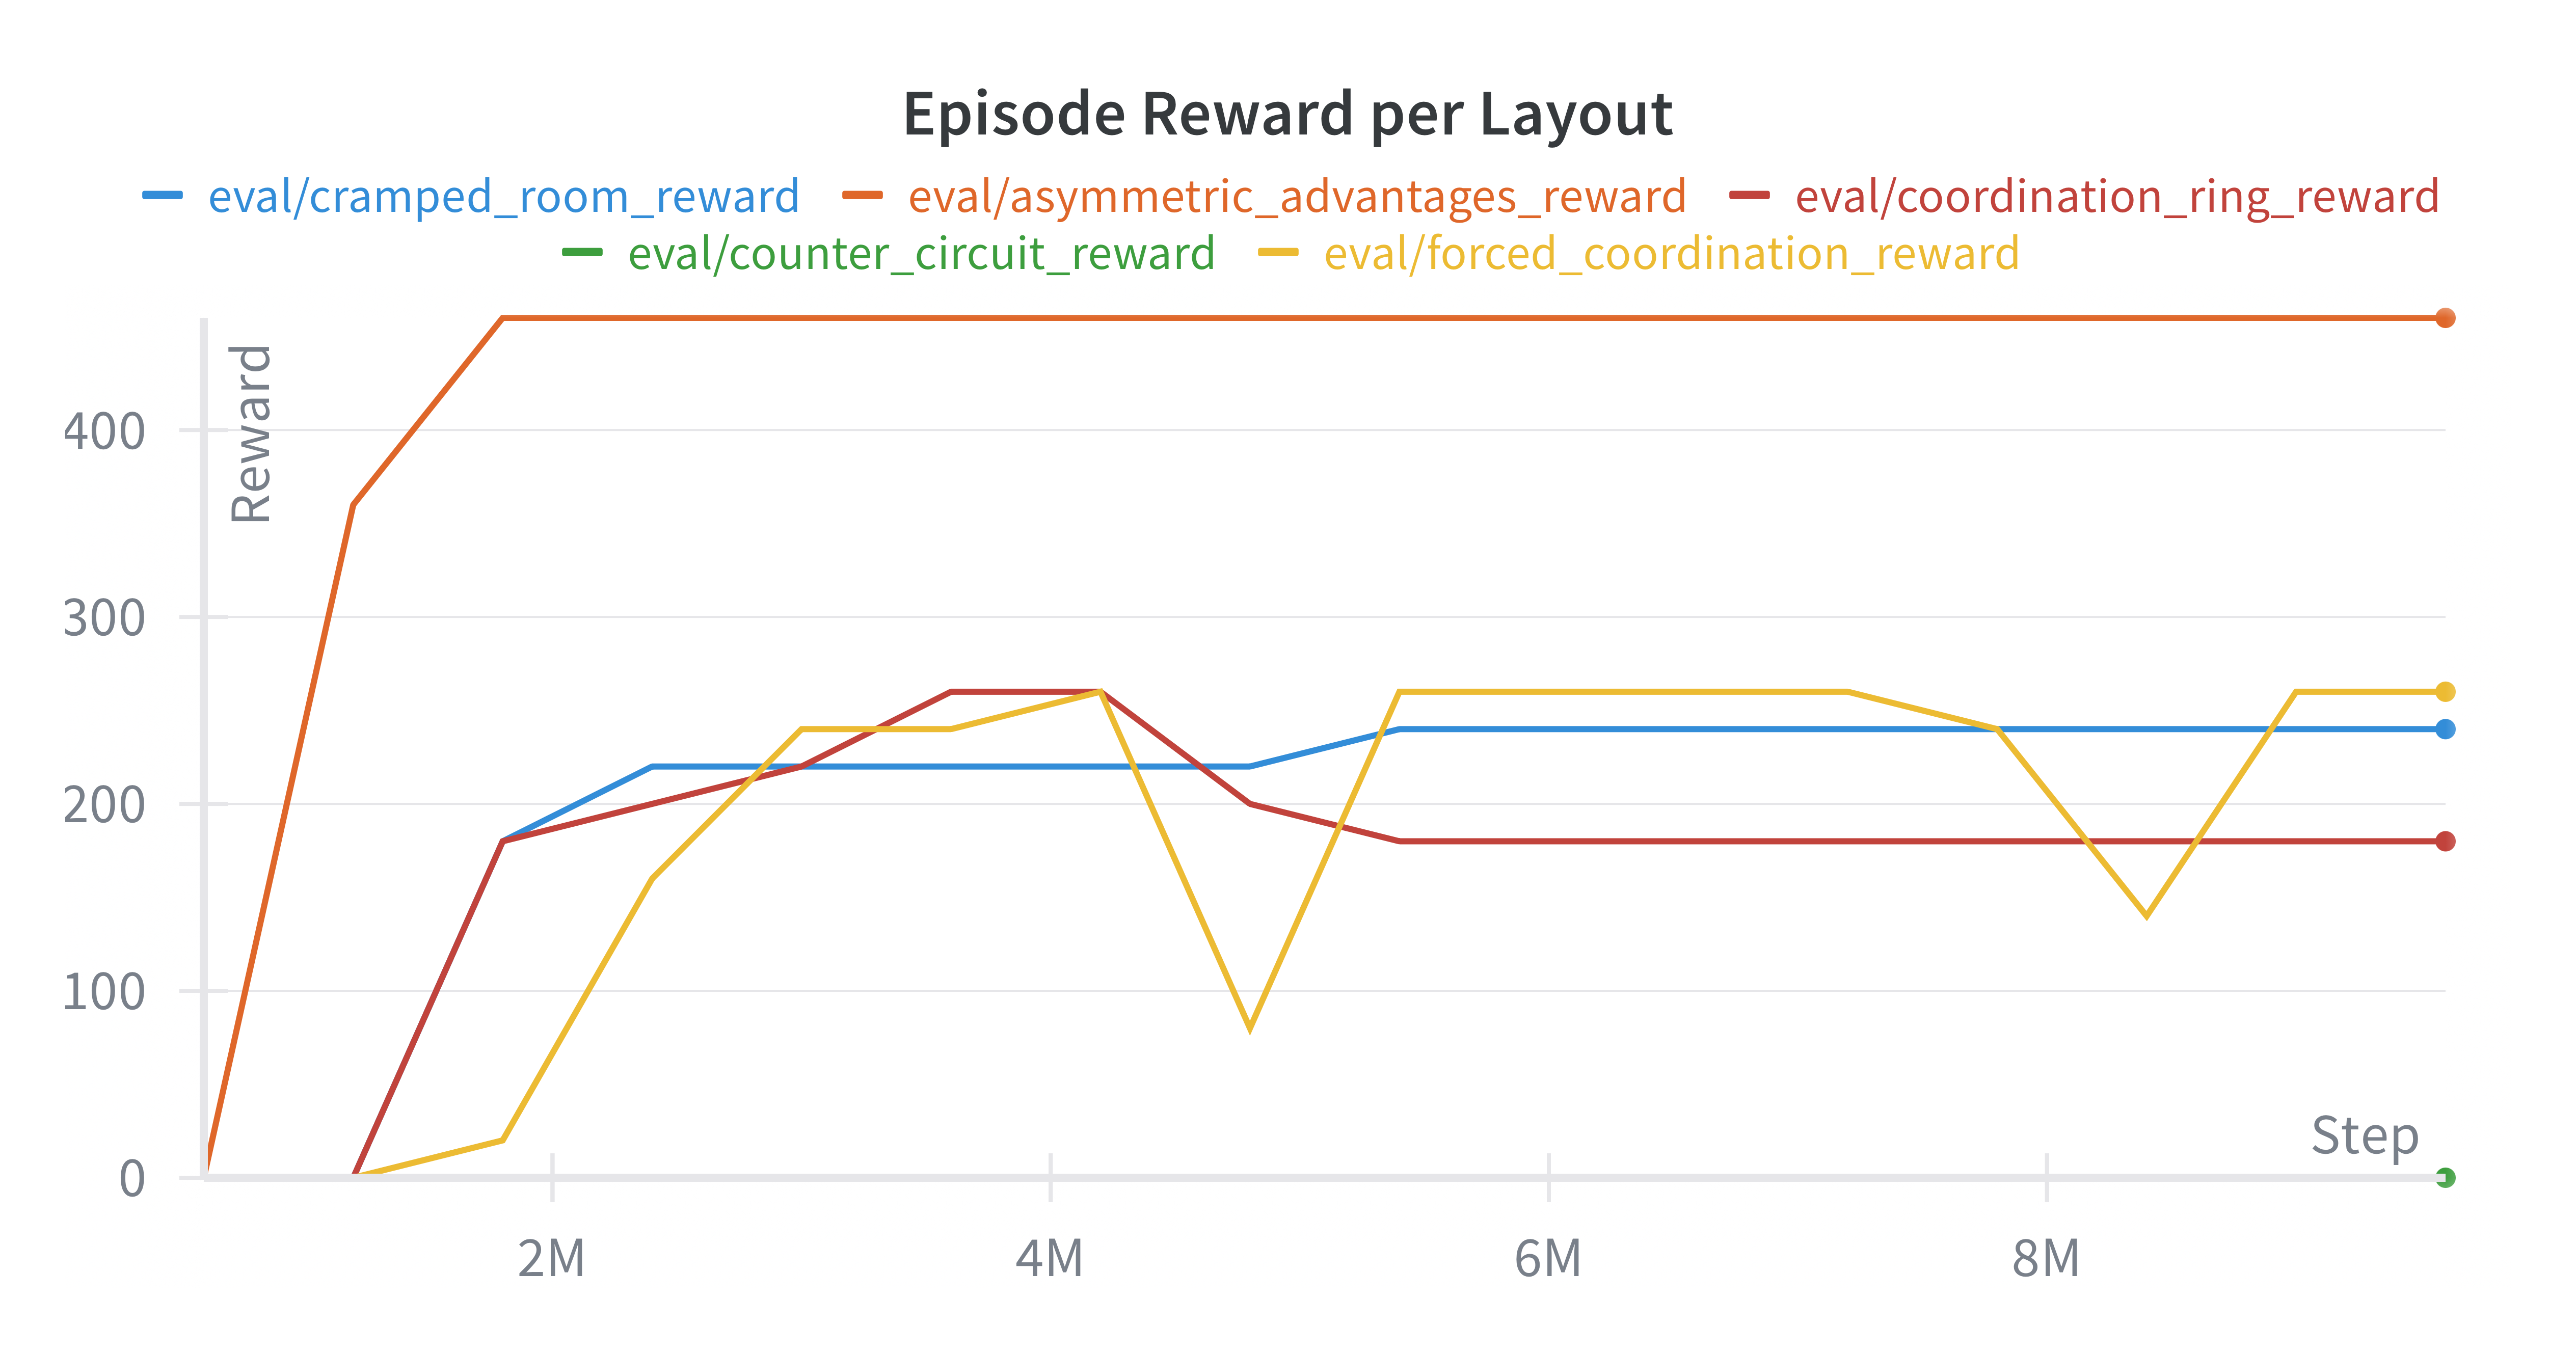
\includegraphics[width=0.75\linewidth]{./images/reward_per_layout_seed_42}
\end{center}

\section{Discussion \& Conclusion}

\bibliographystyle{plain}
\bibliography{references.bib}

\newpage
\appendix
\section{Hyperparameter Optimization Results} \label{appendix:hpo}

\begin{table}[ht]
    \centering
    \small
    \caption{Final hyperparameter configuration determined by Optuna.}
    \label{tab:final_params}
    \begin{tabular}{@{}llll@{}}
        \toprule
        \textbf{Hyperparameter} & \textbf{Type} & \textbf{Search Space}    & \textbf{Best Value} \\
        \midrule
        Network Type            & Categorical   & \{MLP, CNN\}             & MLP \\
        Env Encoding            & Categorical   & \{Featurized, Lossless\} & Featurized \\
        Shared Backbone         & Categorical   & \{True, False\}          & False \\
        MLP Hidden Dim          & Categorical   & \{64, 128, 256\}         & 256 \\
        Learning Rate           & Log-float     & $[10^{-5}, 10^{-3}]$     & $4.5 \times 10^{-4}$ \\
        Entropy Coef            & Log-float     & $[0.01, 0.3]$            & 0.0135 \\
        GAE Lambda              & Float         & $[0.9, 0.99]$            & 0.94 \\
        Update Epochs           & Integer       & $[4, 10]$                & 10 \\
        Num Steps               & Categorical   & \{400, 800\}             & 800 \\
        Parameter Sharing       & Categorical   & \{True, False\}          & True \\
        \bottomrule
    \end{tabular}
\end{table}

\begin{figure}[h]
    \centering
    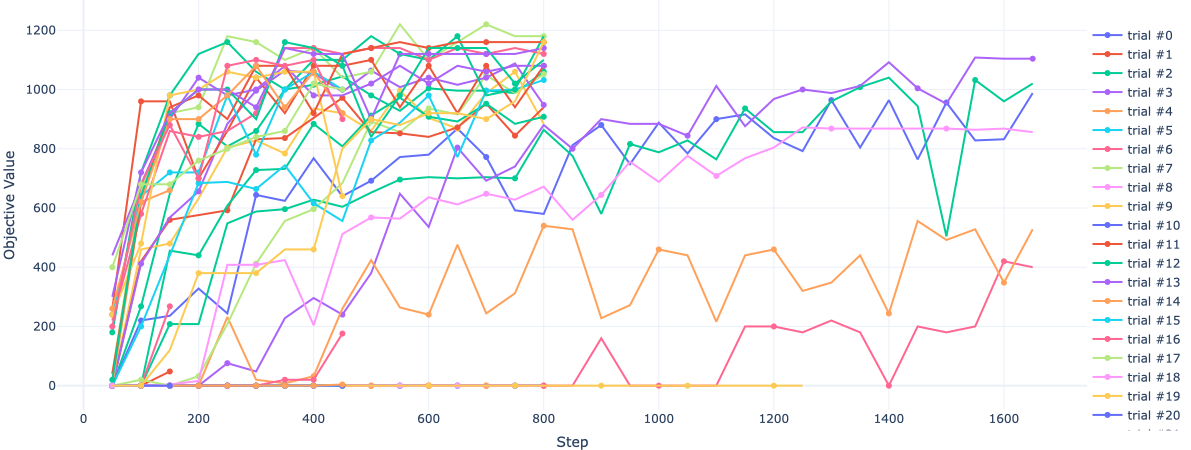
\includegraphics[width=\linewidth]{./images/trials.png}
    \caption{\textbf{Optimization History}: Evolution of objective values
    across 50 trials.}
    \label{fig:opt_history}
\end{figure}

\begin{landscape}
    \begin{figure}[p]
        \centering
        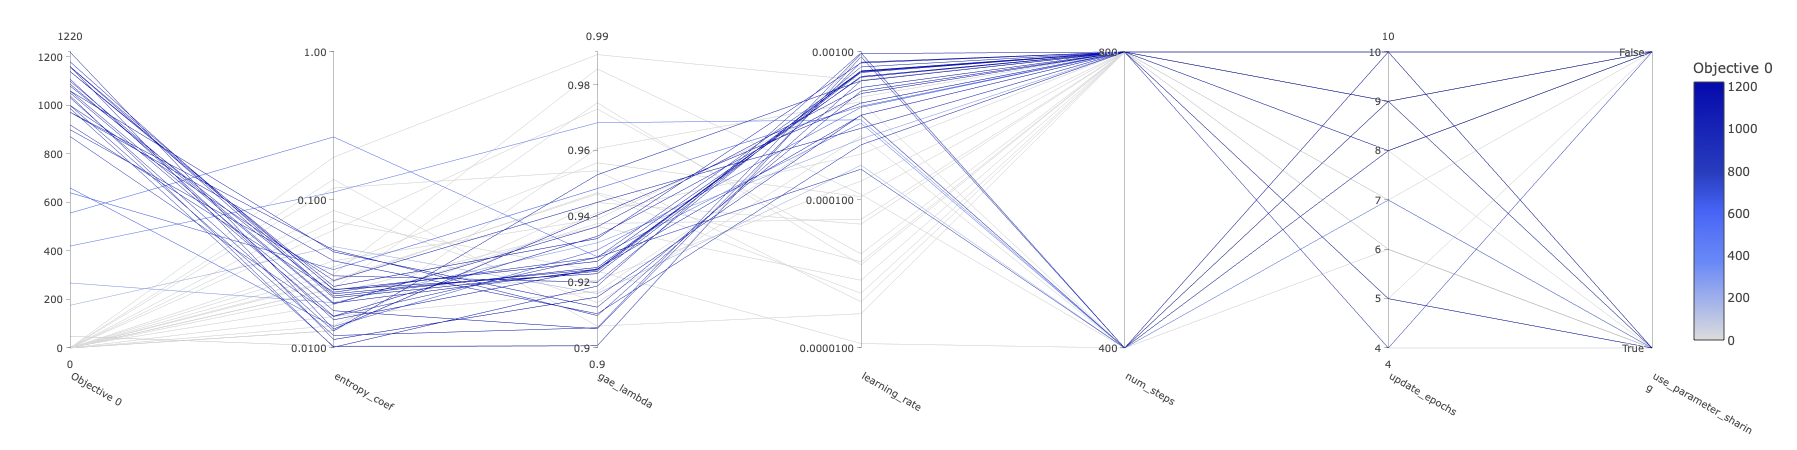
\includegraphics[width=1.0\linewidth]{./images/parallel_coordinate_plot_1.png}
        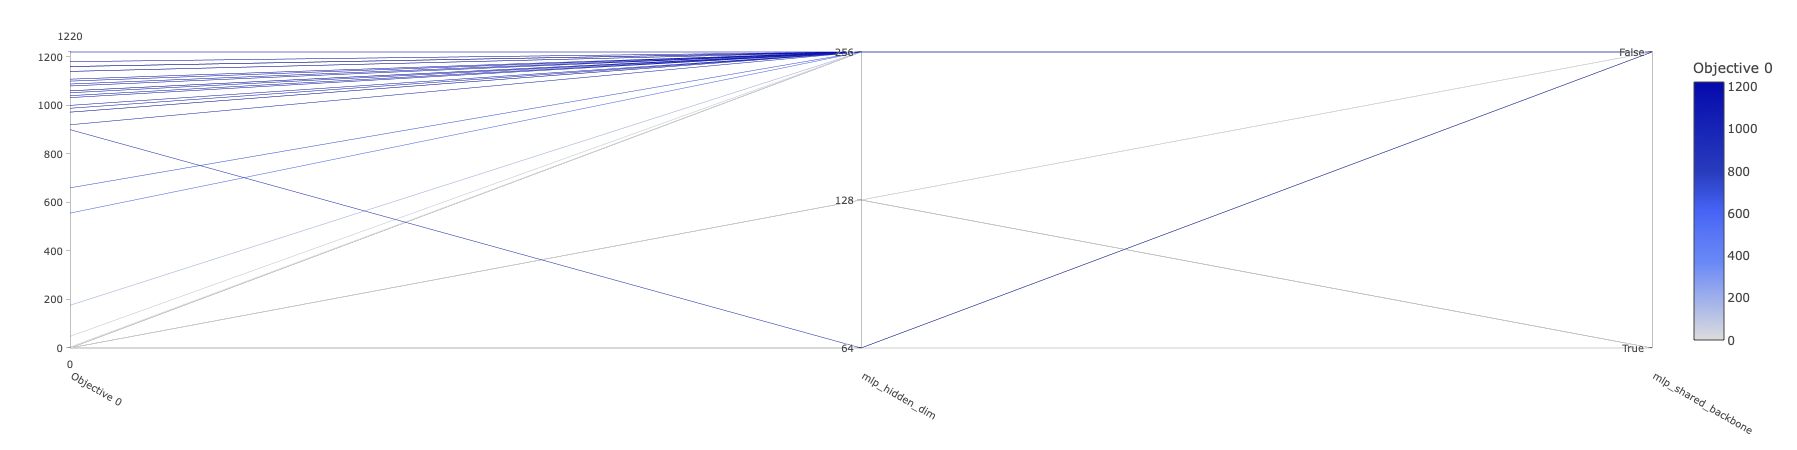
\includegraphics[width=1.0\linewidth]{./images/parallel_coordinate_plot_2.png}
        \caption{\textbf{Parallel Coordinate Plots} illustrating the
            relationship between hyperparameters and total reward. The
            concentration of high-performing trials (dark blue) highlights optimal
        regions for critical hyperparameters.}
        \label{fig:parallel_coords}
    \end{figure}
\end{landscape}

\end{document}
